\subsubsection{Implementation of Steepest Descent}
To better understand the problem at hand the cost function to be minimized is shown in \figref{costFunction}. It might seem strange to do optimization when one could just directly find the minimum by graphical inspection of the cost function. However, this graph took over 5 hours to render and contains the results of \si{90.000} simulations, which makes it a very inefficient and unpractical to work with in general. It is therefore desirable to obtain an optimization algorithm which can give a result in a relatively short time in case of any changes, be it new test data or changes to the system model. In this case the cost function is saved in a data-file, such that it can be plotted during implementation as a graphical reassurance that the optimization algorithm is behaving normally.

\begin{figure}[H]
	\centering
	\includegraphics[width=.55\textwidth]{figures/costFunction2}
	\caption{The cost function to be minimized. The parameters are shown in the xy-plane and the deviation between simulation and test data, cost, for each two parameters is shown on the z axis. To generate the graph 90.000 simulations were run, one for each point on the surface, and the rendering time exceeded 5 hours. This is not practical to work with in general, but valuable in the implementation process of the optimization algorithm.}
	\label{costFunction}
\end{figure}

When implementing the steepest descent method the gradient of the cost function in needed, which includes a numerical differentiation of the model.
%
\begin{flalign}
	\nabla\ P(\vec{\theta}) &= \vec{G}(\vec{\theta}) = \nabla \left( \frac{1}{2N}\sum_{k = 1}^{N} \left(\vec{y}_k - \vec{y}_{m_k}(\vec{\theta})\right)^2 \right) &
\end{flalign}
\begin{flalign}
	\eq{\vec{G}(\vec{\theta})} {- \frac{1}{N} \left(\nabla\ \vec{y}_{m_k}(\vec{\theta})^T(\vec{y}_k - \vec{y}_{m_k}(\vec{\theta})) \right) } &
	\label{gradientOfCostFunction}
\end{flalign}
%
The implementation is seen in \autoref{AlgorithmForModelGradient}.
\begin{lstlisting}[ style=custommatlab,
caption  = {Algorithm for the approximation of the gradient of the cost function.},
label    = AlgorithmForModelGradient ]
%---- CALCULATING THE GRADIENT OF THE COST FUNCTION ------------------------

% gradientOfC = 1/N  * ( Y - Ym ) * Ym' 
% Where:
%   Y      is the data recorded from test
%   Ym     is the model simulation output
%   Ym'    is the partial derivative of the simulated model with respect to
%          each of the parameters to be estimated.

% parameters: J_f B_f
% Small magnitude deviation from these parameters is set
delta = 0.01;

% Calculating the deviation
deltaJ_f = J_f+delta*J_f;
deltaB_f = B_f+delta*B_f;

% Running the simulation again, now with J_f the deviating parameter
deltaYmJf = simCubli( deltaJ_f, B_f, J_f, B_f );

% Running the simulation again, now with B_f as the deviating parameter
deltaYmBf = simCubli( J_f, deltaB_f, J_f, B_f );

% Finally calculating the partial derivatives of the model in (J_f, B_f)
YmDiffBf = ( deltaYmBf - Ym )/ delta;
YmDiffJf = ( deltaYmJf - Ym )/ delta;

% This however is just for the model.. and we need
% the gradient of the cost function, as stated earlier:
% gradientOfC = 1/N  * ( Y - Ym ) * Ym'
gJf = -(1/N)* ((Y - Ym )'*YmDiffJf);
gBf = -(1/N)* ((Y - Ym )'*YmDiffBf);

% The gradient of the cost function in the current point (J_f, B_f) is then:
g = [ gJf
      fBf ];
\end{lstlisting}

With the gradient calculated the search direction is known, and implementation of the forward backward method as described above determines the search interval. This enables the above described Fibonacci line search to minimize the one-dimentional problem in each iteration. In \figref{CostFunctionMinimized3D} the process of the minimization is shown on the cost function and a contour plot is shown in \figref{CostFunctionMinimizedContour}. In the contour plot the black dotted lines shows the search direction and region determined by the gradient and the forward backward method.

\begin{figure}[H]
  \begin{minipage}{\linewidth}
    \captionsetup[subfigure]{font = footnotesize}
    \centering
    \subcaptionbox
    {
      The parameters are shown in the xy-plane and the cost for each set of parameters is shown on the z axis.
      \label{CostFunctionMinimized3D}
    }
    {
      \includegraphics[scale=.5]{costFunctionMinimized2}
    }\quad
    \subcaptionbox
    {
      A contour plot of the cost function with the optimization iterations. Here the black dotted lines shows the search 
      \label{CostFunctionMinimizedContour}
    }
    {
      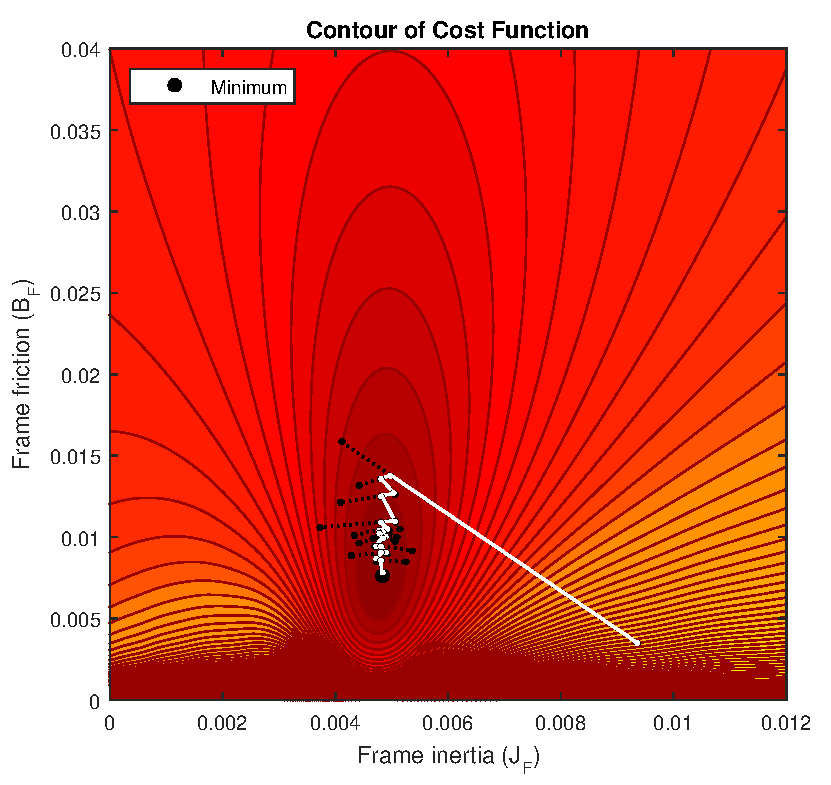
\includegraphics[scale=.5]{costFunctionMinimizedContour}
    }
    \caption{Here each iteration of the steepest descend using Fibonacci and forward backward method is seen directly on the cost function.}
    \label{CostFunctionMinimized}
  \end{minipage}
\end{figure}
%
The final result achieved in by the algorithm is shown in \figref{resultOfGradientWithFibonacciAndForwardBackward}, where the normed RMS error between test results and simulation with final parameters, \si{J_F=4,8 \cdot 10^{-3}\ kg \cdot m^2} and \si{B_F=7,8 \cdot 10^{-3}\ m \cdot s \cdot rad^{-1}}, is also shown.
%
\begin{figure}[H] 
	\centering
	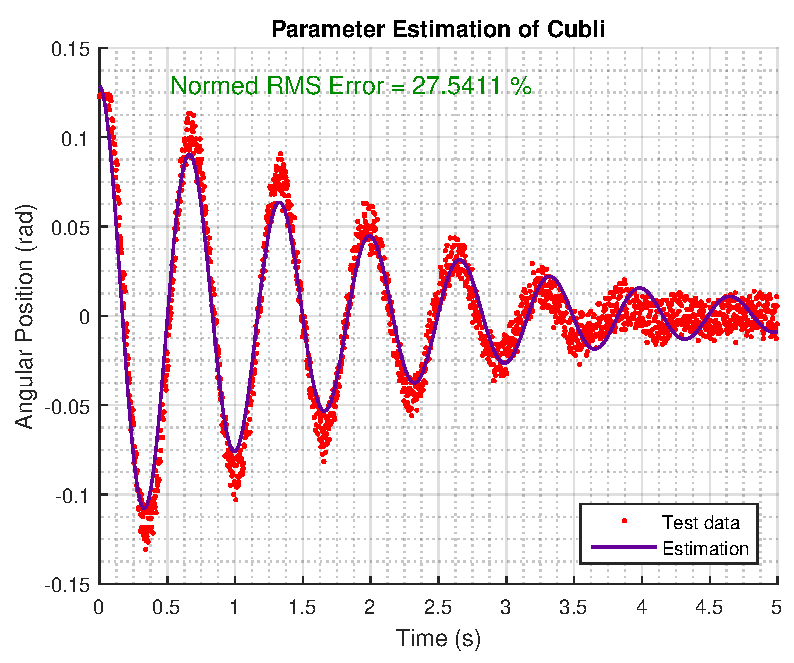
\includegraphics[width=.65\textwidth]{figures/resultOfGradientWithFibonacciAndForwardBackward}
	\caption{The final result of the minimization using steepest descent with Fibonacci line search and forward backward method.}
	\label{resultOfGradientWithFibonacciAndForwardBackward}
\end{figure}